\documentclass[notes,color]{sepslide0}
\usepackage[overheads]{mysepslides}
\usepackage{tech,graphicx,url,tikz,mathsx,scalalistings}
\def\set#1{\{#1\}}
\title{Interacting Peers} 
\author{Gavin Lowe}

% \everymath{\color{Plum}}
\def\smaller{\small} 

\def\scalacolour{\color{violet}}

\begin{document}

\begin{slide}
  
  \Title

Reading: Andrews, Section 7.4.

\end{slide}

%%%%%


\begin{slide}
\heading{Interacting peers}

A common paradigm in concurrent programming is \emph{interacting peers}.
Several threads or processes execute basically the same code, and exchange
messages to achieve some task.  The way in which messages are exchanged can
follow various patterns.
\end{slide}


\begin{slide}
\heading{Interacting peers}

In this chapter we will examine four patterns of interacting peers: 
%
\begin{itemize}
\item
A system with a centralised thread doing most of the work;
\begin{center}
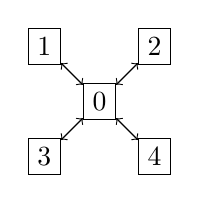
\begin{tikzpicture}[scale = 0.7]
\draw(0,0) node[draw] (0) {0};
\draw(-1,1) node[draw] (1) {1}; \draw[<->] (0) -- (1);
\draw(1,1) node[draw] (2) {2}; \draw[<->] (0) -- (2);
\draw(-1,-1) node[draw] (3) {3}; \draw[<->] (0) -- (3);
\draw(1,-1) node[draw] (4) {4}; \draw[<->] (0) -- (4);
\end{tikzpicture}
\end{center}

\item
A symmetric, fully-connected topology, where each thread sends messages to
all the others;
\begin{center}
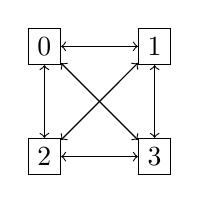
\begin{tikzpicture}[scale = 0.7]
\draw(-1,1) node[draw] (0) {0};
\draw(1,1) node[draw] (1) {1}; 
\draw(-1,-1) node[draw] (2) {2};
\draw(1,-1) node[draw] (3) {3}; 
\foreach \x in {1,...,3}  \draw[<->] (0) -- (\x);
\foreach \x in {2,...,3}  \draw[<->] (1) -- (\x);
\draw[<->] (2) -- (3);
\end{tikzpicture}
\end{center}
\end{itemize}
\end{slide}


\begin{slide}
\heading{Interacting peers}

\begin{itemize}
\item
A ring topology, where each thread communicates with just its two neighbours;
\begin{center}
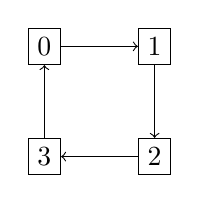
\begin{tikzpicture}[scale = 0.7]
\draw(-1,1) node[draw] (0) {0};
\draw(1,1) node[draw] (1) {1}; 
\draw(-1,-1) node[draw] (3) {3};
\draw(1,-1) node[draw] (2) {2}; 
\draw[->] (0) -- (1); \draw[->] (1) -- (2); 
\draw[->] (2) -- (3); \draw[->] (3) -- (0);
\end{tikzpicture}
\end{center}

\item
A binary tree topology, where each thread communicates just with its parent
and two children.
\begin{center}
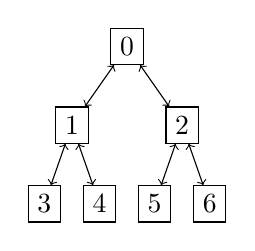
\begin{tikzpicture}[xscale = 0.7, yscale = 1.0]
\draw(0,0) node[draw] (0) {0};
\draw (0)++(-1,-1) node[draw] (1) {1}; \draw[<->] (0) -- (1);
\draw (0)++(1,-1) node[draw] (2) {2}; \draw[<->] (0) -- (2);
\draw (1)++ (-0.5,-1) node[draw] (3) {3}; \draw[<->] (1) -- (3);
\draw (1)++ (0.5,-1) node[draw] (4) {4}; \draw[<->] (1) -- (4);
\draw (2)++ (-0.5,-1) node[draw] (5) {5}; \draw[<->] (2) -- (5);
\draw (2)++ (0.5,-1) node[draw] (6) {6}; \draw[<->] (2) -- (6);
\end{tikzpicture}
\end{center}
\end{itemize}
\end{slide}

%%%%%

\begin{slide}
\heading{The running example}

We will illustrate the patterns with a simple example: at the start, each node
holds an integer; at the end, each node should hold the sum of all those
integers.

For each pattern, we will implement objects implementing the following trait. 
\begin{scala}
/** The trait specifying the various sum examples.
  * Each thread calls apply, passing in its value, and gets back the overall
  * sum. */
trait Sum{
  /** Submit value, and receive back overall sum. 
    * @param me the identity of this thread.
    * @param x the value submitted. */
  def apply(me: Int, x: Int): Int
}
\end{scala}
\end{slide}

%%%%%

\begin{slide}
\heading{Reasoning about patterns}

We will reason about the correctness of the patterns by identifying
\emph{invariants} that hold at certain points in the execution.

We will also consider the \emph{total} number of messages sent.  But this
isn't a good measure of the running time if multiple messages can be sent
concurrently.

Finally, we will consider the number of messages sent \emph{sequentially}.
Recall the ``happens-before'' relation $\preceq$.  We will say that messages
$m_1$, \ldots, $m_n$ form a {\it totally-ordered chain} if
\[
m_1 \prec m_2 \prec \ldots \prec m_n.
\]
We will be interested in identifying the maximum length chain.
\end{slide}

%%%%%

\begin{slide}
\heading{Centralised pattern}

In this protocol, each client node sends its value to a central node, which
calculates the sum, and sends the sum back.

We use a single channel in each direction, which is shared by the client
threads: 
%
\begin{scala}
/** Implementation of Sum using a controller.  The controller is the
  *  thread with identity 0. */
class Centralised(n: Int) extends Sum{
  private val toController = new BuffChan[Int](n-1 max 1)
  private val fromController = new BuffChan[Int](n-1 max 1)

  def apply(me: Int, x: Int): Int = ...
}
\end{scala}
\end{slide}

%%%%%

\begin{slide}
\heading{Centralised pattern}

\begin{scala}
  def apply(me: Int, x: Int): Int = {
    if(me == 0){ // this is the controller
      var sum = x
      // Receive values from other threads
      for(i <- 1 until n){ val w = toController?(); sum += w }
      // Distribute sum
      for(i <- 1 until n) fromController!sum
      sum
    }
    else{
      toController!x     // submit my value
      fromController?() // get back the result
    }
  }
\end{scala}
\end{slide}

%%%%%

\begin{slide}
\heading{Invariant}

Write $x_i$ for the value chosen by node~$i$.  Then during the first stage of
the protocol, the following invariant holds for the controller:
%
\begin{eqnarray*}
\sm{sum} & = & 
   x_0 + \sum \set{x_i \| 1 \le i < n \land 
           \mbox{node~$i$'s value has been received}}.
\end{eqnarray*}
\end{slide}

%%%%%

\begin{slide}
\heading{Efficiency}

This protocol uses $2(n-1)$ messages in total.  However, none of these
messages can occur concurrently, since all messages involve the
controller.

Write $\sm{toController}.i$ for the communication on |toController| from
thread~$i$, and similarly for |fromController|.

We can find a totally-ordered chain of communications
\[
\begin{align}
\mbox{\SCALA{toController}}.i_1 \prec \mbox{\SCALA{toController}}.i_2 
  \prec \ldots  \prec \mbox{\SCALA{toController}}.i_{n-1} \prec \\
\gap
  \mbox{\SCALA{fromController}}.j_1 \prec \mbox{\SCALA{fromController}}.j_2 
  \prec \ldots \mbox{\SCALA{fromController}}.j_{n-1}
\end{align}
\]
for some permutations $i_1, \ldots, i_{n-1}$ and $j_1, \ldots, j_{n-1}$ of $1,
\ldots, n-1$. 
\end{slide}

%%%%%

\begin{slide}
\heading{Testing}

We can test against a sequential specification.  We arrange for each thread to
pick a random value for~|x|, write it into a global array~|xs| (indexed by
thread identities, to avoid race conditions), use the |Sum| object to obtain
the purported sum, and write it to a global array~|results| (again indexed by
thread identities).  We then check that each result was as expected.
\begin{scala}
  val sum = xs.sum
  assert(results.forall(_ == sum), ...)
\end{scala}

See code on course website.
\end{slide}

%%%%%

%% \begin{slide}
%% \heading{Testing}

%% \begin{scala}
%%   /** Array that will hold values chosen by threads, indexed by thread
%%     * IDs. */
%%   var xs: Array[Int] = null

%%   /** Array that will hold results obtained by threads, indexed by thread
%%     * IDs. */
%%   var results: Array[(Int, Int)] = null

%%   /** A thread. */
%%   def thread(me: Int, mm: MinMax) = thread("Thread"+me){
%%     val x = Random.nextInt(1000); xs(me) = x
%%     val (min, max) = mm(me, x)
%%     results(me) = (min, max)
%%   }
%% \end{scala}
%% \end{slide}

%% %%%%%

%% \begin{slide}
%% \heading{Testing}

%% \begin{scala}
%%   /** Run a single test.  */
%%   def runTest = {
%%     val n = 1+Random.nextInt(20) // number of peers
%%     xs = new Array[Int](n); results = new Array[(Int, Int)](n)
%%     val mm = new Centralised(n)
%%     // Run threads
%%     run(|| (for (i <- 0 until n) yield thread(i, mm)))
%%     // Check results
%%     val min = xs.min; val max = xs.max
%%     assert(results.forall(_ == (min, max)),
%%            "xs = "+xs.mkString(", ")+"\nresults = "+results.mkString(", "))
%%   }
%% \end{scala}

%% The main function calls this many times.

%% This is easily adapted to test later patterns. 
%% \end{slide}


%%%%%%%%%%%%%%%%%%%%%%%%%%%%%%%%%%%%%%%%%%%%%%%%%%%%%%%%%%%%


\begin{slide}
\heading{Symmetric or fully-connected pattern}

In this solution, every node sends its value to every other node, which
calculates the sum.

We give each node its own channel on which it can receive messages.
\begin{scala}
/** Implementation of Sum using the symmetric (fully connected) pattern. */
class Symmetric(n: Int) extends Sum{
  /** Channels to send to nodes, indexed by the receivers' identities. */
  private val toNode = Array.fill(n)(new BuffChan[Int](n-1 max 1))

  def apply(me: Int, x: Int): Int = ...
}
\end{scala}
\end{slide}
%%%%% 


\begin{slide}
\heading{Symmetric pattern}

Each node needs to send $\sm{n}-1$ messages, and receive $\sm{n}-1$ messages.
It is easiest if we do these two tasks in parallel.
%
\begin{scala}
  def apply(me: Int, x: Int): Int = {
    /* Thread to send x to other threads. */
    def sender = thread{ for(i <- 0 until n) if(i != me) toNode(i)!x }
    var sum = x // sum so far
    /* Thread to receive from other threads, and accumulate sum. */
    def receiver = thread{
      for(i <- 1 until n){ val w = toNode(me)?(); sum += w }
    }
    run(sender || receiver)
    sum
  }
\end{scala}
\end{slide}

%%%%%


\begin{slide}
\heading{Invariant}

Write $x_j$ for the value chosen by node~$j$.  Then each node~$i$ has a value
for \SCALA{sum} such that:
%
\begin{eqnarray*}
\sm{sum} & = & 
  x_i + \sum \set{x_j \| \mbox{node~$j$ has sent its value to node~$i$}}.
\end{eqnarray*}
\end{slide}

%%%%%

\begin{slide}
\heading{Removing contention}

Each \SCALA{sender} sends to the other nodes in order, starting from
\SCALA{0}.  This means that:
%
\begin{itemize}
\item
All the nodes are contending to send to node~\SCALA{0}, so most will be
temporarily blocked;

\item
Node \SCALA{n-1} has to wait until another node has finished sending to all
other nodes before receiving \emph{anything}.  This gives a chain of length
$2\sm{n}-3$.
\end{itemize}
 
A better way is for each \SCALA{sender} to send in a different order, say
starting from the one with identity one higher than itself:
%
\begin{scala}
def sender = thread{ for(i <- 1 until n) toNode((me+i)%n)!x }
\end{scala}
Now the longest chain is of length $\sm{n}-1$. 
\end{slide}

%%%%%

\begin{slide}
\heading{Efficiency}

This protocol uses $n(n-1)$ messages.  However, they can be sent in just $n-1$
communication rounds (once contention has been removed).
\end{slide}

%%%%%%%%%%%%%%%%%%%%%%%%%%%%%%%%%%%%%%%%%%%%%%%%%%%%%%%%%%%%

\begin{slide}
\heading{A ring topology}

We will see two protocols using a (logical) ring, where each node~$i$ sends
messages to node $(i+1) \bmod n$ and receives from node $(i-1) \bmod n$.
\begin{center}
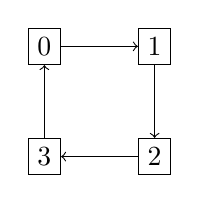
\begin{tikzpicture}[scale = 0.7]
\draw(-1,1) node[draw] (0) {0};
\draw(1,1) node[draw] (1) {1}; 
\draw(-1,-1) node[draw] (3) {3};
\draw(1,-1) node[draw] (2) {2}; 
\draw[->] (0) -- (1); \draw[->] (1) -- (2); 
\draw[->] (2) -- (3); \draw[->] (3) -- (0);
\end{tikzpicture}
\end{center}

In the first protocol, a single token is passed twice round the ring.  

In the second protocol, $n$ tokens are simultaneously passed round the ring. 
\end{slide}

%%%%%

\begin{slide}
\heading{The first ring topology protocol}

The first protocol uses two stages.  During the first stage, node~\SCALA{0}
acts as the initiator, by sending a token containing its value.  

Each node in turn receives the token, which contains the sum so far,
calculates the new sum, including its own value, and sends it on.

More precisely, the value passed from node $i$ to node~$(i+1)
\bmod n$ will equal:
%
\[
\sum \set{x_j \| 0 \le j \le i}.
\]

When the value gets back to node \SCALA{0} it equals the overall sum, 
\[
\sum \set{x_j \| 0 \le j \le n-1}.
\]
This value is then passed around the ring in the second stage, and each node
records the value.
\end{slide}

%%%%%

\begin{slide}
\heading{The first ring topology protocol}

\begin{scala}
/** Implementation of Sum using a ring, with a distinguished initiator.
  * The initiator is the thread with identity 0. */
class Ring(n: Int) extends Sum{
  require(n >= 2)

  /** Channels connecting the threads.  Channel chan(i) goes from thread
    * (i-1)%n to thread i; so thread me receives on chan(me) and sends
    * on chan((me+1)%n). */
  private val chan = Array.fill(n)(new SyncChan[Int])
 
  def apply(me: Int, x: Int): Int = ...
}
\end{scala}
\end{slide}

%%%%%

\begin{slide}
\heading{The first ring topology protocol}

\begin{scala}
  def apply(me: Int, x: Int): Int = {
    val in = chan(me); val out = chan((me+1)%n)
    if(me == 0){                  // This is the initiator
      out!x                       // Start the communications going
      val sum = in?()             // Receive sum back
      out!sum                     // Send it round
      sum
    }
    else{
      val sum1 = in?()            // Receive sum so far
      out!sum1+x                  // Pass on updated values
      val sum = in?()             // Receive final sum
      if(me != n-1) out!sum   // Pass it on
      sum
    }
  } 
\end{scala}
\end{slide}

%%%%%


\begin{slide}
\heading{Efficiency}

This protocol uses $2n-1$ messages, sent sequentially.  Each node is
inactive for most of the time.  This pattern is most effective for problems
where each node can do computation between sending a message and receiving the
next. 

The second ring protocol uses more messages ---a total of $n^2$--- but only
$n$ rounds.  Each node is active for most of the time (so one slow node will
slow down the whole ring).
\end{slide}

%%%%%%%%%%%%%%%%%%%%%%%%%%%%%%%%%%%%%%%%%%%%%%%%%%%%%%%%%%%%

\begin{slide}
\heading{The second ring protocol}

Each value gets passed around the ring.  Each node keeps track of the sum of
values it has seen so far.

More precisely, on its $k$th iteration, each node~$i$ receives a value
from node~$(i-1) \bmod n$ that originated with node $(i-k)\bmod n$; it
sends this value on to node~$(i+1)\bmod n$, and keeps track of the
sum, \SCALA{sum}, it has seen so far:
%
\begin{eqnarray*}
\sm{sum} & = & \sum \set{x_{(i-j)\bmod n} \| 0 \le j \le k}.
\end{eqnarray*}
%
At the end of iteration~$n-1$, it holds the overall sum.
\end{slide}

%%%%%

\begin{slide}
\heading{The second ring protocol}

\begin{scala}
/** Implementation of Sum using a symmetric ring. */
class RingSym(n: Int) extends Sum{
  /** Channels connecting the threads.  Channel chan(i) goes from thread
    * (i-1)%n to thread i; so thread me receives on chan(me) and sends
    * on chan((me+1)%n).  These channels need to be buffered.   */
  private val chan = Array.fill(n)(new BuffChan[Int](1))

  def apply(me: Int, x: Int): Int = ...
}
\end{scala}
\end{slide}

%%%%%

\begin{slide}
\heading{The second ring protocol}

\begin{scala}
  def apply(me: Int, x: Int): Int = {
    val in = chan(me); val out = chan((me+1)%n)
    var sum = x
    out!x                 // send my value round
    for(k <- 1 until n){
      val w = in?()       // receive next value
      sum += w
      out!w               // pass it on
    }
    val w = in?(); assert(x == w) // receive my value back
    sum
  }
\end{scala}
\end{slide}


%%%%%

\begin{slide}
\heading{Buffering}

This protocol needs some buffering between nodes.  Why?

Buffers of size one are enough to ensure correctness.  However, a bit more
buffering might help to overcome inconsistencies in speeds of nodes.
\end{slide}

%%%%%%%%%%%%%%%%%%%%%%%%%%%%%%%%%%%%%%%%%%%%%%%%%%%%%%%%%%%%

\begin{slide}
\heading{Tree-based protocol}

The final protocol works by arranging nodes into a binary tree.  In the
initial stage, values get passed up the tree, starting from the leaves: each
node passes to its parent the sum of the subtree for which it is the root.  At
the end of this stage, the root of the tree obtains the overall sum.  In the
second stage, this value is passed back down the tree.
\end{slide}

%%%%%

\begin{slide}
\heading{Tree-based protocol}

More precisely, we will arrange the nodes into a binary \emph{heap} (as in
heap sort).  Node~$0$ is the root of the tree.  Node~$i$ is the parent of nodes
$2i+1$ and $2i+2$ (if those nodes exist).
\begin{center}
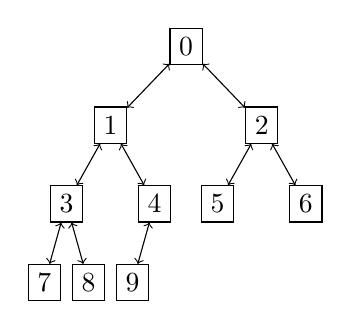
\begin{tikzpicture}[xscale = 0.8, yscale = 1.0]
\draw(0,0) node[draw] (0) {0};
\draw (0)++(-1.2,-1) node[draw] (1) {1}; \draw[<->] (0) -- (1);
\draw (0)++(1.2,-1) node[draw] (2) {2}; \draw[<->] (0) -- (2);
\draw (1)++ (-0.7,-1) node[draw] (3) {3}; \draw[<->] (1) -- (3);
\draw (1)++ (0.7,-1) node[draw] (4) {4}; \draw[<->] (1) -- (4);
\draw (2)++ (-0.7,-1) node[draw] (5) {5}; \draw[<->] (2) -- (5);
\draw (2)++ (0.7,-1) node[draw] (6) {6}; \draw[<->] (2) -- (6);
\draw (3)++ (-0.35,-1) node[draw] (7) {7}; \draw[<->] (3) -- (7);
\draw (3)++ (0.35,-1) node[draw] (8) {8}; \draw[<->] (3) -- (8);
\draw (4)++ (-0.35,-1) node[draw] (9) {9}; \draw[<->] (4) -- (9);
\end{tikzpicture}
\end{center}
\end{slide}

%%%%%

\begin{slide}
\heading{Tree-based protocol}

We will use two arrays of channels, to pass data up and down the tree:
%
\begin{scala}
class Tree(n: Int) extends Sum{
  /** Channels leading up and down the tree.  Each array is indexed by
    * the child's identity. */
  private val up, down = Array.fill(n)(new SyncChan[Int])
  
  def apply(me: Int, x: Int) = ...
}
\end{scala}
%
The arrays are indexed by the \emph{child} node: \SCALA{up(i)} and
\SCALA{down(i)} are used to communicate between node~$i$ and its
parent, node~$(i-1) \div 2$.
\end{slide}

%%%%%

\begin{slide}
\heading{Tree-based protocol}

\begin{scala}
  def apply(me: Int, x: Int) = {
    val child1 = 2*me+1; val child2 = 2*me+2  // identities of children
    var sum = x                                     // sum seen so far
    // Receive sub-sums from both children
    if(child1 < n){ val sum1 = up(child1)?(); sum += sum1 }
    if(child2 < n){ val sum2 = up(child2)?(); sum += sum2 }
    // £sum£ is the sum of values for the subtree rooted at me.
    // Send £sum£ to parent, and wait for overall sum.
    if(me != 0){ up(me)!sum; sum = down(me)?() }
    // Send £sum£ to children
    if(child1 < n) down(child1)!sum
    if(child2 < n) down(child2)!sum
    sum
  }
\end{scala}
\end{slide}




%%%%%

\begin{slide}
\heading{Correctness}

\emph{Claim:} Each node~$i$ (with $0<i<n$) passes to its parent the sum of the
values held by the nodes in the subtree rooted at~$i$:
%
\[
\sum \set{x_j \| j \in descendents(i)}
\]
where
\[
\begin{align}
descendents(i) = \\
\quad
  \set{i} 
    \begin{align}
      \null \union (\If 2i+1<n \mbox{ then } descendents(2i+1) 
      \mbox{ else } \set{}) \\
      \null \union
      (\If 2i+2<n  \mbox{ then }  descendents(2i+2) \mbox{ else } \set{}).
    \end{align}
\end{align}
\]

The claim can be proven by induction on the size of $descendents(i)$.

Hence node~$0$ ends up with the overall sum, which is passed back down the
tree.
\end{slide}

%%%%%

\begin{slide}
\heading{Efficiency}

This protocol uses $2(n-1)$ messages (each node except~0 sends one message on
\SCALA{up}, and receives one message on \SCALA{down}).  It uses about
$4\lfloor \log n \rfloor$ rounds.
\end{slide}

%%%%%

\begin{slide}
\heading{Comparison}

\begin{tabular}{lcc}
Algorithm & messages & rounds \\
\hline
Centralised & $2(n-1)$ & $2(n-1)$ \\
Symmetric & $n(n-1)$ & $n-1$ \\
Ring (1) & $2n-1$ & $2n-1$ \\
Ring (2) & $n^2$ & $n$ \\
Tree & $2(n-1)$ & $\sim 4\lfloor \log n \rfloor$
\end{tabular}
\end{slide}

%%%%%

\begin{slide}
\heading{Summary}

\begin{itemize}
\item
Interacting peers;

\item
Different patterns of interaction: centralised, symmetric, ring, tree;

\item
Reasoning about distributed algorithms;

\item
Efficiency: total number of messages, and number of sequential messages
(rounds).
\end{itemize}
\end{slide}

\end{document}
